\chapter{System architecture}\label{chapter:generalframework}

\section{Different libraries}

The different parts of \smtrat are split into multiple libraries (in the sense of a shared object library) that are responsible for the following tasks:
\begin{itemize}
	\item \code{smtrat-analyzer}: static analysis of input formulae;
	\item \code{smtrat-cad}: back all CAD-based techniques;
	\item \code{smtrat-common}: common definitions and includes;
	\item \code{smtrat-max-smt}: takes care of max SMT queries;
	\item \code{smtrat-mcsat}: utilities for the MCSAT-based solver;
	\item \code{smtrat-modules}: all regular \smtrat modules;
	\item \code{smtrat-optimization}: takes care of optimization queries;
	\item \code{smtrat-qe}: methods for quantifier elimination;
	\item \code{smtrat-solver}: core solving infrastructure;
	\item \code{smtrat-strategies}: strategies for SMT solving;
	\item \code{smtrat-unsat-cores}: takes care of unsat core computations.
\end{itemize}

All of these yield a library, while a full-fledged SMT solver is build from the \sourcepath{cli/} path, in particular the \sourcepath{cli/smtratSolver.cpp}.

\section{Software design}

The architecture of \smtrat puts its focus on modularity and composability of different solving techniques.
Every solving technique, for example SAT solving or the simplex method, is encapsulated in a (derivation of the) \emph{module} class.
These modules are composed to a \emph{strategy} that governs which modules are used in what order.
The execution of a strategy is incumbent upon the \emph{manager}, that also offers an interface for basic SMT solving to the outsi.

More advanced solving techniques like \emph{quantifier elimination}, computing \emph{unsatisfiable cores}, or tackling \emph{max SMT} and \emph{optimization} queries are implemented as individual components in the \emph{frontend}.
The frontend implements (most of) an SMT-LIB compatible interface and can either be used by a generic SMT-LIB \emph{parser}, or an external tool.
This structure is shown in \cref{fig:smtrat-architecture}.

\begin{figure}[ht]
	\centering
	\tikzset{component/.style={draw, text width=2.5cm, align=center, minimum height=0.5cm}}
\tikzset{module/.style={draw, text width=0.75cm, align=center, minimum height=0.5cm}}

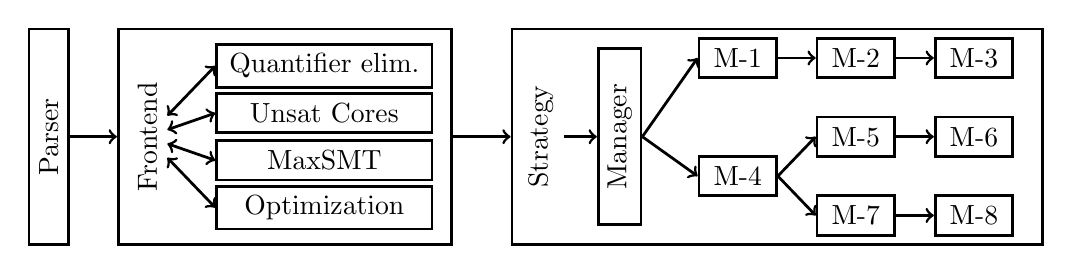
\begin{tikzpicture}[line width=1pt]

	\node[component, rotate=90] (parser) at (-0.25,0) {Parser};

	\node[component, text height=4cm, rotate=90] (frontend-box) at (2.75,0) {};
	\node[rotate=90] (frontend) at (1,0) {Frontend};

	\node[component] (optimization) at (3.25,-0.9) {Optimization};
	\node[component] (maxsmt) at (3.25,-0.3) {MaxSMT};
	\node[component] (unsat-cores) at (3.25,0.3) {Unsat Cores};
	\node[component] (qe) at (3.25,0.9) {Quantifier elim.};

	
	\node[component, text height=6.5cm, rotate=90] (strategy-box) at (9,0) {};
	\node[rotate=90] (strategy) at (6,0) {Strategy};
	\node[component, text width=2cm, rotate=90] (manager) at (7,0) {Manager};

	\node[module] (module1) at (8.5,1) {M-1};
	\node[module] (module2) at (10,1) {M-2};
	\node[module] (module3) at (11.5,1) {M-3};
	\node[module] (module4) at (8.5,-0.5) {M-4};
	\node[module] (module5) at (10,0) {M-5};
	\node[module] (module6) at (11.5,0) {M-6};
	\node[module] (module7) at (10,-1) {M-7};
	\node[module] (module8) at (11.5,-1) {M-8};
	

	\draw[->] (parser) -- (frontend-box);
	\draw[->] (frontend-box) -- (strategy-box);
	\draw[->] (strategy) -- (manager);
	\draw[<->] (frontend) -- (qe.west);
	\draw[<->] (frontend) -- (unsat-cores.west);
	\draw[<->] (frontend) -- (maxsmt.west);
	\draw[<->] (frontend) -- (optimization.west);

	\draw[->] (manager.south) -- (module1.west);
	\draw[->] (module1.east) -- (module2.west);
	\draw[->] (module2.east) -- (module3.west);
	\draw[->] (manager.south) -- (module4.west);
	\draw[->] (module4.east) -- (module5.west);
	\draw[->] (module4.east) -- (module7.west);
	\draw[->] (module5.east) -- (module6.west);
	\draw[->] (module7.east) -- (module8.west);
\end{tikzpicture}
	\caption{Overview of the general \smtrat architecture.}\label{fig:smtrat-architecture}
\end{figure}

The parser itself is implemented in \sourcepath{cli/parser/} and run from \sourcepath{cli/tools/execute_smtlib.h}. The template argument \code{Executor} is usually instantiated with the executor from \sourcepath{cli/tools/Executor.h} which corresponds to the frontend.
The components in the frontend are taken from the respective \smtrat libraries.

The manager is a generic class from \sourcepath{smtrat-solver/Manager.h} that every strategy (from \sourcepath{smtrat-strategies/}) inherits from and only constructs the \emph{strategy graph} in its constructor.
The strategy graph is at the core of the composition of \smtrat modules and \cref{fig:module-in-strategy} shows how a single module is embedded in a strategy.

\begin{figure}[ht]
	\centering
	\tikzset{component/.style={draw, text width=2.5cm, align=center, minimum height=0.5cm}}
\tikzset{module/.style={draw, text width=0.75cm, align=center, minimum height=0.5cm}}

\begin{tikzpicture}[line width=1pt]

	\node (input) at (-3,0) {};
	\node[module] (output1) at (5,1) {B-1};
	\node[module] (output2) at (5,0) {B-2};
	\node[module] (output3) at (5,-1) {B-3};
	\node[component, rotate=90] (received) at (-2,0) {received};

	\node[component, text width=2cm, rotate=90] (passed) at (1.25,0) {passed};

	\node[component, text height=3cm, rotate=90] (module-box) at (0,0) {};
	\node[align=left, anchor=north west] (module) at ($(module-box.north east)$) {Module};


	\draw[->] (input) -- (received);
	\draw[->] (passed) -- node[sloped, above, pos=0.6] {condition-1} (output1.west);
	\draw[->] (passed) -- node[sloped, above, pos=0.6] {condition-2} (output2.west);
	\draw[->] (passed) -- node[sloped, above, pos=0.6] {condition-3} (output3.west);
\end{tikzpicture}
	\caption{One \smtrat module in a strategy.}\label{fig:module-in-strategy}
\end{figure}

Every module has (a pointer to) a set of \emph{received formulae} that represent its input and a set of \emph{passed formulae} that represent the formula that is passed on to some backend.
The module may ``solve'' the query from its input on its own, or it may pass (one or more) queries to its \emph{backends} (in this case B-1, B-2 and B-3).
Arrows to backends may be labeled with \emph{conditions} that restrict whether this particular backend can be used, for example checking whether the passed formulae are linear, contain integer variables or bit-vector formulae.

When a module issues a backend call the manager identifies all suitable backend modules (where the condition evaluates to true) and calls all backend modules on the passed formulae. This happens either sequentially (until one backend module solves the query) or in parallel.

\section{Modules}
A module $m$ holds a set of formulas, called its \emph{set of received formulas} and denoted by $\Crcv(m)$. The main function of a module is \texttt{check(bool full)}, which either decides whether $\Crcv(m)$ is satisfiable or not, returning \SAT or \UNSAT, respectively, or returns \UNKNOWN. A set of formulas is semantically defined by their conjunction. If the function's argument \texttt{full} is set to \false, the underlying procedure of $m$ is allowed to omit hard obstacles during solving at the cost of returning \UNKNOWN in more cases. We can manipulate $\Crcv(m)$ by adding (removing) formulas $\varphi$ to (from) it with \texttt{add($\varphi$)} (\texttt{remove($\varphi$)}). Usually, $\Crcv(m)$ is only slightly changed between two consecutive \texttt{check} calls, hence, the solver's performance can be significantly improved if a module works incrementally and supports backtracking. In case $m$ determines the unsatisfiability of $\Crcv(m)$, it has to compute at least one preferably small \emph{infeasible subset} $\Cinf(m)\subseteq \Crcv(m)$. Moreover, a module can specify \emph{lemmas}, which are valid formulas. They encapsulate information which can be extracted from a module's internal state and propagated among other modules. Furthermore, a module itself can ask other modules for the satisfiability of its \emph{set of passed formulas} denoted by $\Cpass(m)$, if it invokes the procedure \texttt{runBackends(bool full)} (controlled by the manager). It thereby delegates work to modules that	 may be more suitable for the problem at hand. 

\section{Strategy}
\label{sec::strategy}
\smtrat allows a user to decide how to compose the modules. For this purpose we provide a graphical user interface, where the user can create a \emph{strategy} specifying this composition. A strategy is a directed tree $T:=(V, E)$ with a set $V$ of modules as nodes and $E\subseteq V\times \Omega\times\Sigma\times V$, with $\Omega$ being the set of \emph{conditions} and $\Sigma$ being the set of \emph{priority values}. A condition is an arbitrary Boolean combination of formula properties, such as propositions about the Boolean structure of the formula, e.g., whether it is in conjunctive normal form (CNF), about the constraints, \eg whether it contains equations, or about the polynomials, e.g., whether they are linear. Furthermore, each edge carries a unique priority value from $\Sigma=\{1,\ \ldots,\ |E|\}$.

\section{Manager}
\label{sec::manager}
The \emph{manager} holds the strategy and the SMT solver's input formula $C_{input}$. Initially, the manager calls the method \texttt{check} of the module $m_r$ given by the root of the strategy with $\Crcv(m_r) = C_{input}$. Whenever a module $m\in V$ calls \texttt{runBackends}% for its passed formula $\Cpass(m)$
, the manager adds a \emph{solving task} $(\sigma,\ m,\ m')$ to its priority queue $Q$ of solving tasks (ordered by the priority value), if there exists an edge $(m,\ \omega,\ \sigma,\ m')\in E$  in the strategy such that $\omega$ holds for $\Cpass(m)$. If a processor $p$ on the machine where \smtrat is executed on is available, the first solving task of $Q$ is assigned to $p$ and popped from $Q$. The manager thereby starts the method \texttt{check} of $m'$ with $\Crcv(m') = \Cpass(m)$ and passes the result (including infeasible subsets and lemmas) back to $m$. The module $m$ can now benefit in its solving and reasoning process from this shared information. Note that a strategy-based composition of modules works incrementally and supports backtracking not just within one module but as a whole. This is realized by a mapping in each module $m$ of its passed formulas $\varphi\in\Cpass(m)$ to sets $R_1,\ldots,\ R_n \subseteq \Crcv(m)$ such that each $R_i$ forms a reason why $m$ included $\varphi$ in $\Cpass(m)$ to ask for its satisfiability. In order to exploit the incrementality of the modules, all parallel executed backends terminate in a consistent state (instead of just being killed), if one of them finds an answer.
  
\section{Procedures implemented as modules}
\label{sec:implemented_modules}
The heart of an SMT solver usually forms a SAT solver. In \smtrat, the module \satModule abstracts $\Crcv(\satModule)$ to propositional logic and uses the efficient SAT solver \minisat~\cite{minisat} to find a Boolean assignment of the abstraction. It invokes \texttt{runBackends} where $\Cpass(\satModule)$ contains the constraints abstracted by the assigned Boolean variables in a less-lazy fashion~\cite{sebastiani2007lazy}. The module \simplexModule implements the Simplex method equipped with branch-and-bound and cutting-plane procedures as presented in \cite{DM06}. We apply it on the linear constraints of any conjunction of \supportedLogics constraints. For a conjunction of nonlinear constraints \smtrat provides the modules \gbModule, \vsModule and \cadModule, implementing GB~\cite{JLCA_CAI13}, VS~\cite{Article_Corzilius_FCT2011} and CAD~\cite{Article_Loup_TubeCAD} procedures, respectively. Moreover, the module \icpModule uses ICP similar as presented in~\cite{GGIGSC10}, lifting splitting decisions and contraction lemmas to a preceding \satModule and harnessing other modules for nonlinear conjunctions of constraints as backends. The exact procedure is going to be published. The module \cnfModule invokes \texttt{runBackends} on $\Cpass(\cnfModule)$ being the CNF of $\Crcv(\cnfModule)$, and the module \ppModule performs some preprocessing based on factorizations and sum-of-square decompositions of polynomials.

\section{Infeasible subsets and lemmas}
\label{sec::infsubset_lemmas}
Infeasible subsets and lemmas, which contain only formulas from
$\Cpass(\SATM)$ of a preceding \SATM, prune its Boolean search space and hence the number of theory calls. 
Smaller infeasible subsets are usually more advantageous, because they make larger cuts 
in the search space. We call lemmas containing new constraints \emph{inventive lemmas} (\emph{non-inventive} otherwise). 
They might enlarge the Boolean search space, but they can reduce the complexity of later theory calls.
When using inventive lemmas, it is important to ensure that the set possible
constraints introduced in such lemmas is finite for a given module and a given 
input formula. Otherwise, the termination of this procedure cannot be guaranteed. In general, any module might contribute lemmas 
and all preceding modules in the solving hierarchy can directly involve them in their search for satisfiability.
